\section*{Alert-policy evaluation}
The discrimination table summarizes all three splits. Boosting has the highest mean AUROC in A; the GRU has the highest mean AUROC in B. These are descriptive rankings: the seed-specific test populations overlap. Average precision remains low, and the class-weighted models are not calibrated probabilities. Full patient-bootstrap intervals and Brier scores are in the appendix.
\begin{table}[t]
\centering\small\setlength{\tabcolsep}{4pt}
\caption{Pre-onset discrimination, mean across three seeds. AP denotes average precision. Per-seed 95\% patient-bootstrap intervals appear in the seed-specific uncertainty table; seed averaging is not an independent-cohort meta-analysis.}

\begin{tabular}{lrrrr}\toprule
Model & AUROC A & AUROC B & AP A & AP B\\\midrule
Logistic & 0.745 & 0.666 & 0.049 & 0.025 \\
Boosting & 0.794 & 0.731 & 0.060 & 0.033 \\
GRU & 0.778 & 0.752 & 0.060 & 0.031 \\
\bottomrule\end{tabular}\end{table}


For every model and seed, the local A and B calibrations certify grid infeasibility at $\alpha=0.05$, for every tested budget from 0.1 to 1 review per patient. There are 90 local calibration/budget outcomes; each certificate retains its stated per-grid confidence interpretation. The result concerns the frozen grids, not all thresholds or all monitoring designs. Increasing review capacity cannot repair a grid whose first-alert timing already violates the risk target.

\begin{figure*}[t]
\centering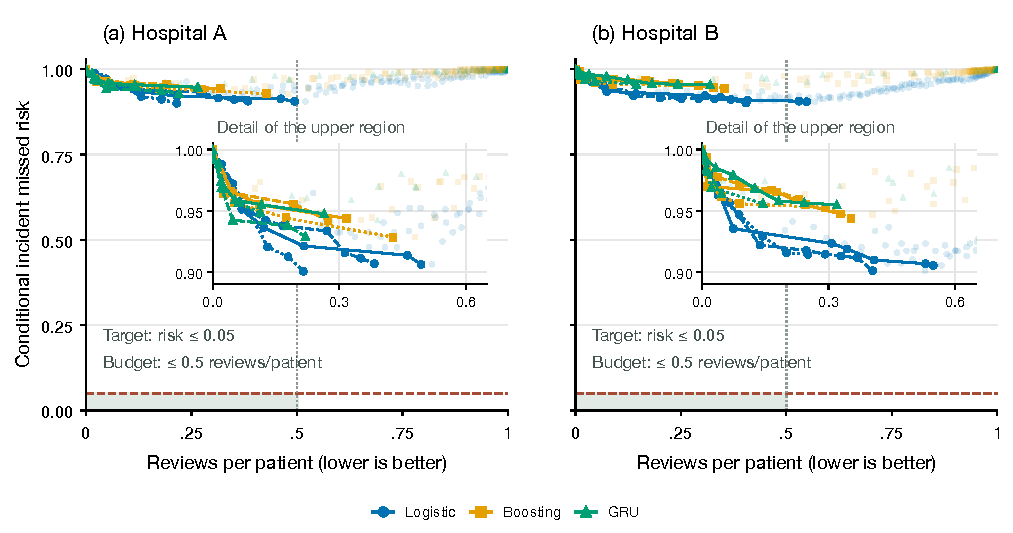
\includegraphics[width=\linewidth]{figs/risk_workload_detailed.pdf}
\caption{The tested first-alert grids remain far from the target region. All three seeds are shown (solid, dashed and dotted), with faint markers for dominated thresholds. Each model has 51 validation-quantile candidates plus endpoints before deduplication. Lines are frontier guides, not attainable interpolations. Shading marks risk $\le0.05$ and workload $\le0.5$. Panels show hospitals A and B; each inset enlarges risk 0.89--1.0 while the outer axes retain the complete risk range.}

\end{figure*}

The risk–workload figure also shows the realized test risks. Even the best test-grid point, selected retrospectively only to describe the frontier, misses at least 90.0\% of eligible incidents. This stringent endpoint treats a review just before the six-hour window as a miss, even if it might be useful clinically. The negative result is therefore about timely \emph{first} review under this definition, not about whether early alerts have clinical value.

We additionally choose thresholds by validation challenge utility and freeze them before testing (the operating-policy table). Boosting in A achieves mean utility 0.332 with 0.193 reviews per patient, yet its strict incident missed risk is 0.960. Its three test splits contain 742 eligible incident observations in total, counting overlap across splits: 414 receive an early first alert and 298 receive none before onset. Only 30 receive their first alert in the specified window. The challenge utility credits a broader time window and a persistent positive state; it is not a surrogate for this first-review endpoint.

Repeated alerts recover more incidents but require several reviews per patient. At validation-selected utility thresholds, no model/site/policy combination has all three of positive utility, risk at most 0.05, and workload at most 0.5. This is the empirical answer to the declared joint target, not proof against alternative cooldown or continuing-review policies.
\begin{table*}[t]
\centering\small
\caption{Validation-selected operating policies, means over three seeds. ``Repeated'' reviews every above-threshold hour. Utility uses full-stay states; risk and review count use the retrospective pre-onset endpoint. No test metric chooses a threshold.}
\label{tab:policies}
\begin{tabular}{lllrrr}\toprule
Model & Site & Policy & Missed risk & Reviews/patient & Utility\\\midrule
Logistic & A & First & 0.936 & 0.215 & 0.333 \\
Logistic & A & Repeated & 0.298 & 8.077 & 0.342 \\
Logistic & B & First & 0.916 & 0.296 & 0.085 \\
Logistic & B & Repeated & 0.302 & 10.185 & 0.003 \\
Boosting & A & First & 0.960 & 0.193 & 0.332 \\
Boosting & A & Repeated & 0.318 & 6.741 & 0.380 \\
Boosting & B & First & 0.970 & 0.091 & 0.125 \\
Boosting & B & Repeated & 0.494 & 4.162 & 0.183 \\
GRU & A & First & 0.949 & 0.160 & 0.347 \\
GRU & A & Repeated & 0.406 & 6.124 & 0.352 \\
GRU & B & First & 0.971 & 0.081 & 0.155 \\
GRU & B & Repeated & 0.534 & 4.172 & 0.180 \\
\bottomrule\end{tabular}\end{table*}


\begin{figure*}[t]
\centering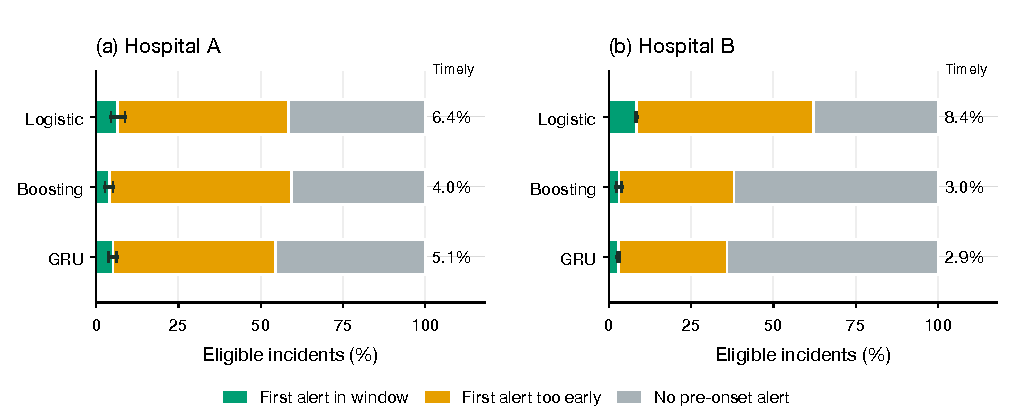
\includegraphics[width=\linewidth]{figs/first_alert_outcomes.pdf}
\caption{First-alert failures come from both early reviews and absent reviews. Bars show mean fractions across three seed-specific test sets at validation-utility-selected thresholds. Dark whiskers span the minimum and maximum timely fraction across seeds; they are descriptive ranges, not confidence intervals. Each label at the right gives the mean timely fraction.}

\end{figure*}

The first-alert outcomes figure separates the two mechanisms. An earlier review is not equivalent to an unreviewed patient, but both fail the strict first-review window. This decomposition should accompany any interpretation of the aggregate missed-risk value.

Local B calibration contains 230--242 eligible positives, compared with 219--253 in A. None of 14,400 overlapping calibration subsets (25, 50, 100 or 200 positives) certifies the 5\% first-alert risk target. Thus the fraction of test-risk violations \emph{among certified rules} is undefined, not zero. Four hundred positives are unavailable in these calibration pools; the study does not establish how much additional data would suffice. All 72 prespecified group/model/site/seed checks also exclude their tested grids.

Consent interventions do not restore feasibility. They change both scores and the descriptive fallback threshold, so a reduced review count need not be an improvement. For example, GRU opt-out at 50\% per feature group changes mean A missed risk from 0.952 to 0.979 while reviews fall from 0.207 to 0.104 per patient. These are simulated permissions, not observed patient preferences. The estimated-ratio repeated-alert diagnostic has external-site risk from 0.034 to 0.152 across model/seed combinations and carries no exact shift guarantee.

The corrected reviewer audit evaluates 972 queue scenarios on frozen scores. Across all these scenarios, end-to-end missed risk ranges from 0.912 to 0.987; a perfect reviewer cannot recover an incident that never receives a timely review. The simulation is not evidence about real clinician performance. Among 500 random DAGs, 126 contain a source-to-action path and 103 contain a path bypassing the randomly assigned review nodes. This illustrates why review nodes alone do not enforce review, while remaining a synthetic structural test.


\begin{figure*}[t]
\centering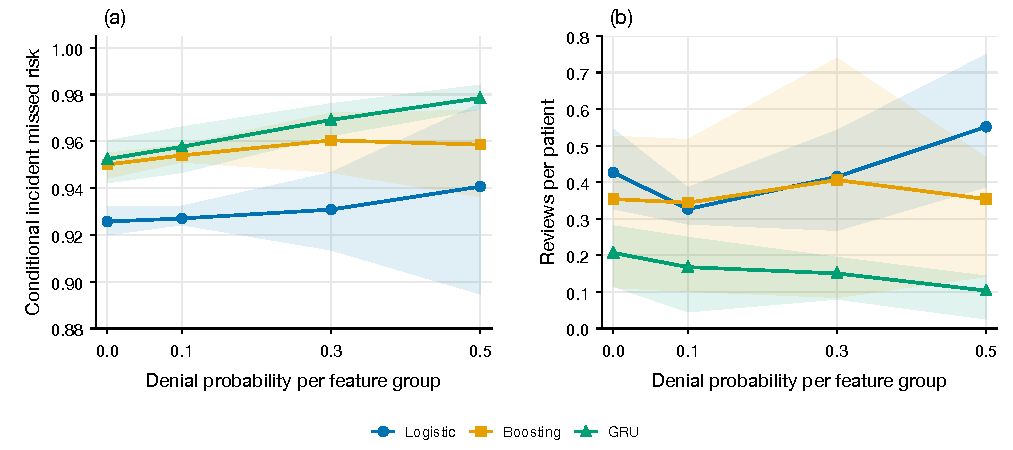
\includegraphics[width=\linewidth]{figs/consent_cost.pdf}
\caption{Admission opt-out changes incident risk and review demand together. Hospital A results use independently denied lab and vital groups and scenario-specific calibration-selected empirical fallback thresholds. Lines are three-seed means; shading spans the observed seed range. Panel (a) uses an expanded high-risk scale, not a zero baseline. No point carries a certified consent-scenario risk guarantee.}

\end{figure*}

The consent-cost figure shows why fewer reviews cannot be interpreted in isolation. The GRU's review demand falls as more input groups are denied, while its already high missed risk increases. Logistic and boosting responses are less monotone because permission changes alter the score trajectories and the empirical fallback threshold. The released revocation analysis additionally separates admission opt-out from clearing state at hour 12. Neither intervention recovers a certified first-alert operating point.
